\section{图(Graphs)和会话(Session)}
TensorFlow用数据流图(dataflow graph)代表操作间的相应的计算。这导致首先你需要先定义图,创建TensorFlow Session通过本地设备或远程设备运行图的一部分。这个向导对于你想用低级变量模型是很有用的。要记得像tf.estimator.Estimator和Keras中的API对于用户端隐藏了图和会话的细节。
\subsection{为什么用数据流图?}
数据流图对于并行编程来说是一个常见的模型。在数据流图中,节点(node)代表了计算单元,边(edge)代表了数据消耗和产生。例如在TensorFlow图中,tf.matmul操作将对应两个边(两个相乘的矩阵)单个节点一个输出(相乘的结果)。
TensorFlow利用数据流图计算有如下好处:
\begin{itemize}
\item 并行性:通过指定边代表不同操作间的依赖,系统能很容易的识别能并行执行的操作。
\item 分布执行:通过用边代表值在不同操作间的流动,这对于tensorflow分割你的程序到不同的机器上的设备(CPUs,GPUs,TPUs)上,TensorFlow插入必须的计算和不同设备间的协调。
\item 编译:TensorFlow的XLA compiler可以用你的数据流图的信息生成更快的代码,例如通过融合连接操作。
\item 数据流图是一个代表你模型的代码,你可以用Python建立图,存储在SavedModel,为了更低的推理延迟在C++程序中恢复。
\end{itemize}
\subsection{建立一个tf.Graph}
大多数的TensorFlow的开始阶段构造一个数据流图,在这个阶段,你利用TensorFlow的API函数构造tf.Operation(节点)和tf.Tensor(边)对象,添加它们到图实例上。TensorFlow提供默认的图到相同上下文环境下的API函数,例如:
\begin{itemize}
\item 调用tf.constant(42.0)创建一个tf.Operation生成值42.0,添加值到默认的图上,返回一个代表这个常量值的tf.Tensor。
\item 调用tf.matmul(x,y)创建一个tf.Tensor对象x,y用tf.Operation相乘,增加它到默认的图上,返回一个代表相乘结果的tf.Tensor。
\item 执行 v=tf.Variable(0)给图添加一个tf.Operation到图上,操作将存储可以写的Tensor值在tf.Session.run调用前。tf.Variable对象包装这个操作,然后它能被像tensor一样使用,Tensor将读取当前存储的值。tf.Variable对象有assign和assign\_add之类的方法,当方法被执行的时候,更新存储的值。
\item 调用tf.train.Optimizer.minimize将操作和tensor添加到默认的图上计算梯度,返回一个tf.Operation,当运行的时候,用图读设置变量。
\end{itemize}
多数程序依赖于默认的图,在TensorFlow API调用大多数程序仅仅添加操作和tensor到默认的图上,并不执行实际的计算。当你通过这些tf.Tensor和tf.Operation代表你的函数传递给tf.Session进行计算。
\subsection{命名你的操作}
tf.Graph对象给它包含的包含tf.Operation对象定义了一个namespace。TensorFlow自动为你图上的操作选择一个独一无二的名字,而且给操作名字使程序易读和方便调试。TensorFlow API提供了两个操作来覆盖操作的名字:
\begin{itemize}
\item 每个API函数创建一个新的tf.Operation或者返回一个新的tf.Tensor时接受一个name选项。例如tf.constant(42.0,name="answer")创建一个新的操作名字叫answer,返回一个名字为”answer:0“的tf.Tensor。如果默认图已经包含了名字为"answer"的操作,TensorFlow将添加"-1","-2"等等,例如:
\begin{python}
c_0 = tf.constant(0,name="c")#操作的名字为"c"
c_1 = tf.constant(2,name="c")#操作的名字为"c_1"
with tf.name_scope("outer"):
    c_2 = tf.constant(2,name="c")#操作的名字为outer/c
    with tf.name_scope("inner"):
        c_2 = tf.constant(3,name="c")
    c_4 = tf.constant(4,name="c")#操作名字为"outer/c_1"
    with tf.name_scope("inner"):
        c_5 = tf.constant(5,name="c")
\end{python}
\end{itemize}
tf.Tensor对象隐藏为tf.Operation名字,之后tf.Operation将产生tensor作为输出。一个tensor的名字形式"<OP\_NAME>:<i>",这里:
\begin{itemize}
\item "<OP\_NAME>"是产生它的操作的名字。
\item "<i>"是一个整数操作输出的tensor的索引。
\end{itemize}
\subsection{放置操作在不同的设备上}
如果你想TensorFlow用多个不同的设备,tf.device函数提供了方便的方法请求所有的操作在一个特别的上下文被放置现在相同的设备上。
指定格式如下:
\begin{python}
/job:<JOB_NAME>/task:<TASK_INDEX>/device:<DEVICE_TYPE>:<DEVICE_INDEX>
\end{python}
这里:
\begin{itemize}
\item <JOB\_NAME>是一个alpha数字,不是以数字开头
\item <DEVICE\_TYPE>是一个注册的设备。
\item <TASK\_INDEX>一个非负整数代表job中的任务的索引
\item <JOB\_NAME>查看tf.train.ClusterSpec查看更多关于jobs和tasks的解释。
\item <DEVICE\_INDEX>:一个代表device索引的非负整数,例如为了区别在同一进程中的不同GPU。
\end{itemize}
你不需要指定设备的每一部分,例如,如果你运行在一个单GPU的机器上,你也许用tf.device添加一些操作到CPU和GPU上。
\begin{python}
weights = tf.random_normal()
with tf.device("/device:CPU:0")
    img = tf.decode_jpeg(tf.read_file("img.jpg"))
with tf.device("/device:GPU:0"):
    result = tf.matmul(weights,img)
\end{python}
如果你用典型的分布式配置部署TensorFlow,你也许指定job的名字和task ID放置变量在参数服务器job("/job:ps"),其它的操作在worker job("/job:worker")
\begin{python}
with tf.device("/job:ps/task:0"):
    weight_1 = tf.Variable(tf.truncated_normal([784,100]))
    biases_1 = tf.Variable(tf.zeros([100]))
with tf.device("/job:ps/task:1"):
    weight_2 = tf.Variable("/job:ps/task:1"):
    biases_2 = tf.Variable(tf.zeros([10]))
with tf.device("/job:worker"):
    layer_1 = tf.matmul(train_batch,weight_1)+biases_1
    layer_2 = tf.matmul(train_batch,weight_2)+biases_2
\end{python}
tf.device给你很高的灵活度度选择放置单个操作或者更广范围的TensorFlow图。在一些情况下,有简单的算法。例如tf.train.replica\_device\_setter API可以用tf.device防止操作data-parallel distributed training.例如下面的代码段显示tf.train.replica\_device\_setter应用不同的放置策略到tf.Vriable对象和其它操作:
\begin{python}
with tf.device(tf.train.replica_device_setter(ps_tasks=3)):
# tf.Variable objects are, by default, placed on tasks in "/job:ps" in a
# round-robin fashion.
    w_0 = tf.Variable(...)  # placed on "/job:ps/task:0"
    b_0 = tf.Variable(...)  # placed on "/job:ps/task:1"
    w_1 = tf.Variable(...)  # placed on "/job:ps/task:2"
    b_1 = tf.Variable(...)  # placed on "/job:ps/task:0"
    input_data = tf.placeholder(tf.float32)     # placed on "/job:worker"
    layer_0 = tf.matmul(input_data, w_0) + b_0  # placed on "/job:worker"
    layer_1 = tf.matmul(input_data, w_1) + b_1  # placed on "/job:worker"
\end{python}
\subsection{Tensor-like对象}
一些TensorFlow操作接受一个或者更多的tf.Tensor对象作为参数。例如,tf.matmul得到tf.Tensor对象,tf.add\_n得到一个tf.Tensor列表对象。为了方便使用这些函数在tf.Tensor中接受一个tensor-like对象,用tf.convert\_to\_tensor方法转换它为tf.Tensor,Tensor-like包含下面的元素类型:
\begin{itemize}
\item tf.Tensor
\item tf.Variable
\item numpy.ndarray
\item list(tensor-like对象的列表)
\item Python标量:bool,float,int,str。
\end{itemize}
你可以用tf.register\_tensor\_convension\_function。

默认,每次你的相同的tensor-like对象TensorFlow将创建一个新的tf.Tensor。如果tensor-like对象很大(numpy.ndarray包含一些训练样本),当你多次使用你也许会超出内存。为了避免这样,手动调用tf.convert\_to\_tensor在tensor-like对象,用tf.Tensor返回。
\subsection{在tf.Session执行图}
TensorFlow用tf.session类代表客户程序(通常是Python程序),通过一个类似的接口在(C++也可用),一个tf.Session对象提供访问在本地机器上的设备,远程设备用分布式的TensorFlow域。它也缓存一些关于你的tf.Graph的信息以至于你能高校的运行相同的计算多次。
\subsection{创建tf.Session}
如果你用低层的TensorFlow API,你可以为当前图创建一个tf.Session
\begin{python}
#创建一个默认的session
with tf.Session() as sess:
#创建一个远程会话
with tf.Session("grpc://example.org:2222"):
\end{python}
因为一个tf.Session拥有自己的物理资源(像GPU和网络连接),它是典型用作上下文管理(with)自动关闭会话。但是你应该确定调用tf.Session.close当你完成后你必须释放资源。

高级API像tf.train.MonitoredTrainingSession或者tf.estimator.Estimator将创建和管理一个tf.Session给你。APIs接受target和config参数(或者作为tf.estimator.RunConfig的一部分),含义如下:
tf.Session.\_\_init\_\_接受三个参数:
\begin{itemize}
	\item target 如果这个参数为空,会话仅仅用在本地机器上。然而,你也许指定grpc:// URL指定TensorFlow Server地址让会话访问server上的所有设备。查看tf.train.Server查看TensorFlow创建server的详细信息。例如通常between-graph replication配置,tf.Session在同一进程中作为客户连接tf.train.Server。
	\item graph 默认情况下新的tf.Session将被限制到仅能在当前的图上运行操作。如果你在你的程序中用多个图,你可以在创建会话的时候指定tf.Graph。
	\item config 这个参数允许你指定tf.Configproto控制session的行为。例如包含一些配置选项。
	\item allow\_soft\_placement 设置设个参数为True使用soft 设备放置算法,该算法忽略tf.device注释尝试放置CPU-only操作在GPU设备。
	\item cluster\_def:当用分布式的TensorFlow,这个选项允许你指定用于计算的机器,提供不同job名字的映射任务索引和网络地址。
	\item graph\_option.optimizer\_options:在执行前提供控制优化TensorFlow的执行。
	\item gpu\_options.allow\_grouth:设置为True改变GPU内存分配因至于它的随着内存分配渐渐增长,而不是启动的时候分配尽量多的内存。
\end{itemize}
\subsection{用tf.Session.run执行操作}
tf.Session.run是运行tf.Operation和评估tf.Tensor的主要操作,一可以传递一个或者更多的tf.Operation和tf.Tensor或者tensor-like 类型的对象,像tf.Variable。这些fetch决定了tf.Graph的使用于计算fetch的所有子图操作的输出。例如下面的代码片段显示了不同的参数能操作不同的子图执行:
\begin{python}
x = tf.constant([[37.0,-23.0],[1.0,4.0]])
w = tf.Variable(tf.random_uniform([2,2]))
y = tf.matmul(x,w)
output = tf.nn.softmax(y)
init_op = w.initializer
with tf.Session() as sess:
#初始化变量
    sess.run(init_op)
    print(sess.run(output))
    y_val,output_val = sess.run([y,output])
\end{python}
tf.Session.run也可以用feeds字典,字典映射tf.Tenor(典型的tf.placeholder())对象为合适执行的值(典型的Python标量,列表,Numpy数组)。
\begin{python}
x = tf.placeholder(tf.float32,shape=[3])
y = tf.square(x)
with tf.Session() as sess:
    print(sess.run(y,{x:[1.0,2.0,3.0]}))
    print(sess.run(y,{x:[0.0,0.0,5.0]}))
    #sess.run(y) 运行z此代码会Raise  `tf.errors.InvalidArgumentError`
    #因为当你计算一个tensor的时候它以来的值应该给定。
    #sess.run(y,{x:37.0})Raises `ValueError`,因为37.0的形状不匹配
\end{python}
tf.Session.run也接受一个选项options参数使你指定调用的选项,run\_metadata参数使你收集关于执行的metadata。例如你可以用下面的选项处理执行信息:
\begin{python}
y = tf.matmul([[37.0,-23.0],[1.0,4.0]],tf.random_uniform([2,2]))
with tf.Session() as sess:
	#定义sess.run的选项
    options = tf.RunOptions()
    options.output_partition_graphs = True
    options.trace_level = tf.RunOptions.FULL_TRACE
#定义返回metadata的容器
metadata = tf.RunMetadata()
sess.run(y,options=options,run_metadata=metdadata)
#打印每个设备执行的子图
print(metadata.partition_graphs)
\end{python}
\subsection{GraphDef和MetaGraphDef}
TensorFlow用数据流图作为程序的表示,一个tf.Graph包含两个相关的信息:
\begin{itemize}
\item 图的结构(Graph structure):节点和边指示了操作如何被组合在一起。但是没有描述它们如何被使用,图的结构像集合代码,查看它们可能传达一些有用的信息,但是它不包含源代码传送的所有信息。
\item 图集合(Graph collections)TensorFlow提供了一个通常的机制从tf.Graph的恢复metadata集合。tf.add\_to\_collection函数使得你能用key(tf.GraphKeys定义的一些标准的key)结合列表对象看,tf.get\_colletion使得你能结合key查看所有的对象,一些TensorFlow库用如下机制:当你创建一个tf.variable,它被增加到代表全局变量和和训练的变量集合中,之后你创建一个tf.train.Saver或者tf.train.Optimizer,集合中的变量被用作默认参数。
\end{itemize}
一个图可以用两种形式表示:
\begin{itemize}
	\item tf.GraphDef:合适图结构的低级表示,包含所有操作的描述和它们之间的边。tf。GraphDef代表使用的低级APIs,像tensorflow:session C++ APIs 通常它要求额外的上下文环境(如典型的操作的名字)来充分使用它。tf.Graph.as\_graph\_def方法转换一个tf.Graph为tf.GraphDef。
	\item tf.train.MetaGraphDef:这是数据流图的高级表示它包含一个tf.GraphDef,和一些帮助我们理解图的信息(像图集合的上下文信息)。tf.train.export\_meta\_graph函数转化一个tf.Graph为tf.trainMetaGraphDef。tf.train.Saver.save方法也写一个\newline tf.train.MetaGraphDef,它可能被用在结合保存的checkpoint文件去恢复训练保存点的状态。
\end{itemize}
通常情况下我们鼓励你用tf.train.MetaGraphDef而不是tf.GraphDef。在一些情况下tf.GraphDef是很有用的,例如当用下tf.import\_graph\_def或者Graph Transform这样的低级函数修改图,但是tf.train.MetaGraphDef建议用于高级应用。例如用tf.train.MetaGraphDef SavedModel library包装tf.Graph和一系列训练模型参数以至于它们能被后续服务使用。

如果你有tf.train.MetaGraphDef,tf.train.import\_meta\_graph函数将载入默认的图,调用这个函数有下面两种特征:
\begin{itemize}
	\item 它将从原始的图集合中恢复图的内容。像tf.global\_variable和默认的参数像 \newline tf.train.latest\_checkpoint 函数可能被用于从类似的checkpoint目录寻找最新的checkpoint
\end{itemize}
如果你有一个tf.GraphDef,tf.import\_graph\_def函数使得你能载入图进一个已经存在的pythont f.Graph对象。为了利用导入的图,你必须知道在tf.GraphDef中操作或者Tensor的名字。tf,import\_graph\_def函数有两个主要的特性帮你用导入的图:
\begin{itemize}
	\item 你可以通过传递选项input\_map参数重新绑定导入图的tensor对象到默认的图。例如,input\_map使你获取定义在tf.GraphDef导入图的片段,连接图中的tensor和你在代码段中创建的tf.placeholder。
	\item 你可以传递它们的名字到return\_elements列表从导入的图中返回tf.Tensor或者tf.Operation对象
\end{itemize}
\subsection{可视化你的图}
TensorFlow提供一个工具帮助你理解你图中的代码。图的可视化是tensorBoard
的一个组件它在你的浏览器中生成你的图的结构。最简单的创建可视化的方法是当创建tf.summary.FileWriter时传递tf.Graph
\begin{python}
# Build your graph.
x = tf.constant([[37.0, -23.0], [1.0, 4.0]])
w = tf.Variable(tf.random_uniform([2, 2]))
y = tf.matmul(x, w)
# ...
loss = ...
train_op = tf.train.AdagradOptimizer(0.01).minimize(loss)
with tf.Session() as sess:
# `sess.graph` provides access to the graph used in a `tf.Session`.
    writer = tf.summary.FileWriter("/tmp/log/...", sess.graph)
# Perform your computation...
for i in range(1000):
    sess.run(train_op)
      # ...
writer.close()
\end{python}
注意当你用tf.estimator.Estimator时,图(上面的任何总结)将被自动采集到你创建estimator时指定的model\_dir。
你可以在TensorBoard中打开采集,导航到Graph,查看你的图的高级可视化结果。注意典型的TenmsorFlow图,特别是训练图自动计算梯度,同一时间有很多节点可视化。图可视化操作利用scope的名字分组相关的操作到高级节点。你可以点击橙色的+按钮展开里面的子图。
\begin{figure}[H]
	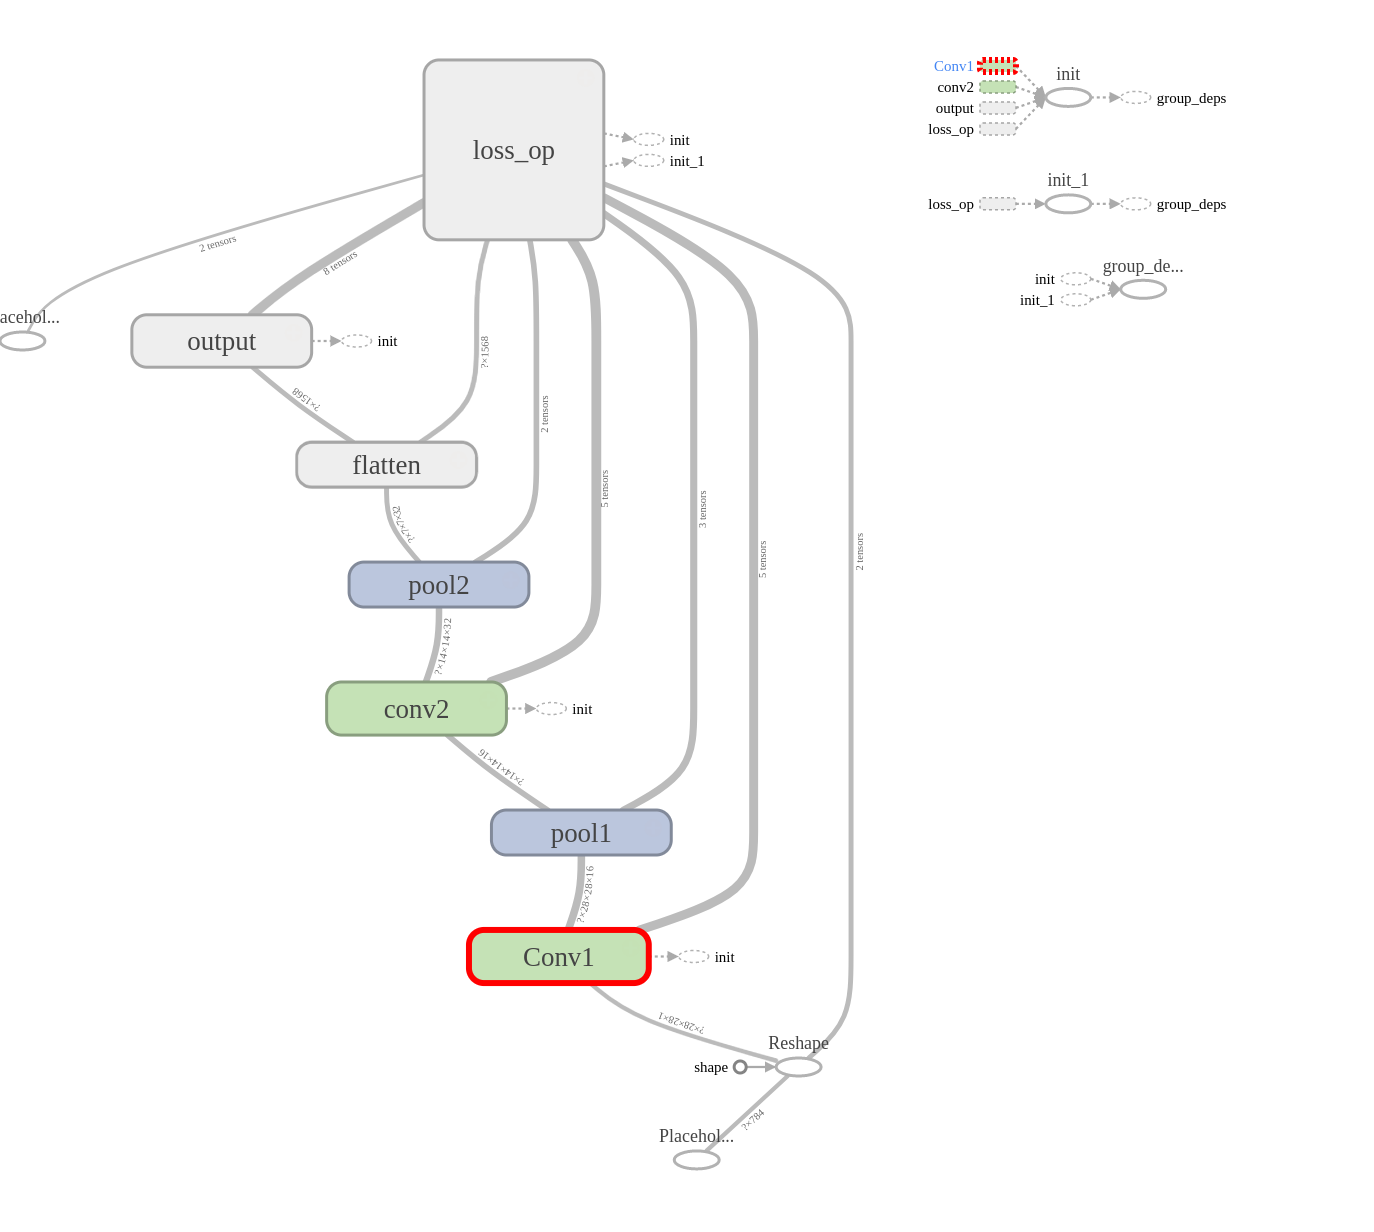
\includegraphics[scale=0.3]{mnist_cnn.png}
\end{figure}
\subsection{用多图编程}
注意当训练一个模型的时候,通常的使用你的代码的方式是用一个图训练你的模型,另一个图评估或者在你的训练好的模型执行推理。在一些情况下,推理图将不同于训练图,例如像dropout,batch normalization在不同的情况下用不同的操作。更进一步,默认的程序像tf.train.Saver用tf.Variable对象的名字在不同的checkpoint中的变量中识别。当用这种方式编程的时候,你可以完全用Python处理建立,执行图,你也可以在同一进程用多个图。TensorFlow提供了一个默认的图隐含的在相同的上下文环境传递所有的API函数。对于一些程序,单个图是足够的,然而tensorFlow也提供了方法操作默认的节点,下面的情况下可能很有用:
\begin{itemize}
	\item 一个tf.Graph为tf.Operation对象定义了tf.Operation的namespace,每个图中的操作必须有独一无二的名字。TensorFlow将第一无二的名字通过添加"\_1","\_2"形成,因此如果它们的名字已经被传出去了,用多个操作创建图给你对操作的名字更好的控制。
	\item 默认的图存储关于每个tf.Operation和tf.Tensor的信息。如果你的程序创建了很多互不连接的子图,用不同的tf.Graph建立子图可能更高效,因此不相关的状态可能被垃圾收集器收集。
\end{itemize}
你可以安装一个不同的tf.Graph作为默认的图,用tf.Graph.as\_default上下文管理器:
\begin{python}
g_1 = tf.Graph()
with g_1.as_default():
    c = tf.constant("Node in g_1")
    sess_1 = tf.Session()
g_2 = tf.Graph()
with g_2.as_default():
    d = tf.constant("Node in g_2")
sess_2 = tf.Session(graph=g_2)
assert c.graph is g_1
assert sess_1.graph is g_1
assert d.graph is g_2
assert sess_2.graph is g_2
\end{python}
查看当前默认的图可以使用tf.get\_default\_graph返回一个tf.Graph对象。
\begin{python}
# Print all of the operations in the default graph.
g = tf.get_default_graph()
print(g.get_operations())
\end{python}
